\documentclass{article}
\usepackage{hyperref} % used for links
\usepackage{listings}
\usepackage{circuitikz}
\usepackage{tikz}
\usepackage{xstring}
\usepackage{amsmath}
\usepackage{graphicx}

%--------------------Make usable space all of page
\setlength{\oddsidemargin}{0in}
\setlength{\evensidemargin}{0in}
\setlength{\topmargin}{0in}
\setlength{\headsep}{-.25in}
\setlength{\textwidth}{6.5in}
\setlength{\textheight}{8.5in}

\lstset{language=C, basicstyle=\ttfamily, breaklines=true}

% Hyperlink setup
\hypersetup{
	colorlinks=true,
	linkcolor=blue,
	filecolor=magenta,      
	urlcolor=cyan,
}

% circuitikz shapes ---------------
\makeatletter
% create the shape (switch without arrow) 
\pgfcircdeclarebipole{}{\ctikzvalof{bipoles/interr/height 2}}{spst}{\ctikzvalof{bipoles/interr/height}}{\ctikzvalof{bipoles/interr/width}}{
	
	\pgfsetlinewidth{\pgfkeysvalueof{/tikz/circuitikz/bipoles/thickness}\pgfstartlinewidth}
	
	\pgfpathmoveto{\pgfpoint{\pgf@circ@res@left}{0pt}}
	\pgfpathlineto{\pgfpoint{.6\pgf@circ@res@right}{\pgf@circ@res@up}}
	\pgfusepath{draw}   
}

% make the shape accessible with nice syntax
\def\pgf@circ@spst@path#1{\pgf@circ@bipole@path{spst}{#1}}
\tikzset{switch/.style = {\circuitikzbasekey, /tikz/to path=\pgf@circ@spst@path, l=#1}}
\tikzset{spst/.style = {switch = #1}}
\makeatother
% --------------------------------

% MATH -------------------------------------
% Vertical vector
\newcommand{\vvec}[1]{\begin{pmatrix} #1 \end{pmatrix}}

\begin{document}
	
	\tableofcontents
	\newpage
	
	\section{Setup of the project}
		\subsection{Hardware used}
		We used an Arduino Nano ATmega328, bought at \href{http://nl.rs-online.com/}{rs-components}.
		
		We used a \href{http://www.mijn-gadgets.nl/Webwinkel-Product-157562595/ENC28J60-Ethernet-Shield-Network-Module-V1.0-For-Arduino-Nano.html}{ENC28j60 Ethernet shield}, the version specifically for the nano. This seemed easier than a wifi shield because of this reason, and with a wifi shield it seemed we needed extra components and a circuit, and we didn't really understand it.
		
		\subsubsection{Components list}
			\begin{itemize}
				\item BC547 NPN transistor
				\item BC557 PNP transistor
				\item $4.7$k $\Omega$ resistor (yellow - violet - red - gold)
				\item $1$k $\Omega$ resistor (brown - black - black - brown - brown - red)
				\item $10$k $\Omega$ resistor (brown - black - orange - gold)
			\end{itemize}
	
		\subsubsection{Button circuit}
			We implemented the begin- and endstops in the circuit for the buttons that move the panels up and down. When a button is NOT pushed, 1 and 1B, and 2 and 2B of that button are connected. When a button is pushed, connections are made between 1 and 1A, and 2 and 2A of that button.
			\begin{center}\begin{circuitikz}
				\draw 
				% 20, 28, E4
					(4,0) node {20} 
					(6,0) node {28}
					(8,0) node {E4}
					
				% button hoog
					(0.75 , -6) node {button up}
					(2.25, -5.25) node {1A}
					(2.25, -6) node {1}
					(2.25, -6.75) node {1B}
					(3.75, -5.25) node {2A}
					(3.75, -6) node {2}
					(3.75, -6.75) node {2B}
				
				% button laag
					(10 ,-6) node {button down}
					(7.25, -5.25) node {1A}
					(7.25,-6) node {1}
					(7.25, -6.75) node {1B}
					(8.5, -5.25) node {2A}
					(8.5, -6) node {2}
					(8.5, -6.75) node {2B}
					
				% drawing
					% 28 to 1,2 hoog via eindstoppen
						(6,-0.25) to (6,-1)
							to (3,-1) 
							to (3,-2)
						(2.5,-2) to (3.5,-2)
						(2.5,-2) to[switch, l_= high end stop] (2.5,-4) %eindstop hoog
							to (1.75,-4)
							to (1.75,-6) to (2,-6) 
						(3.5,-2) to[switch = low end stop] (3.5,-4) %eindstop laag
							to (4.25,-4)
							to (4.25,-6) to (4,-6) 
					% 1A hoog to 1B laag
						(2,-5.25) to (1.9,-5.25)
							to (1.9,-4.75)
							to(5.75,-4.75)
							to(5.75,-6.75)
							to(7,-6.75)
					% 2B hoog to 1A laag
						(4,-6.75) to (5.25,-6.75)
							to (5.25,-5.25)
							to (7,-5.25)
					% 20 to 1 laag
						(4,-0.25) to (4,-1.25)
							to (6.25,-1.25)
							to (6.25,-6)
							to (7,-6)
					% 1 laag to 2 laag
						(7.5,-6) to (8.25,-6)
					% E4 to 2A laag
						(8,-0.25) to (8,-4.75)
							to (9,-4.75)
							to (9,-5.25)
							to (8.75,-5.25)
				;
			\end{circuitikz}\end{center}
			
		\subsubsection{Arduino circuit}
			\begin{center}\begin{circuitikz}
				\draw[dashed] 
					(2,10) to (5,10)
						to (5,14)
						to (2,14)
						to (2,10)
					(3.5,13) node[align=left] {Lenze\\ frequency\\ inverter}
				;
				\draw
				%E4 and its components (Arduino I/O, transistors)
					(10,0) node {E4}
					(1,1.225) node[align=center] {Arduino\\ I/O}
					(10,2) node [pnp] (pnpE4) {}
						(pnpE4.B) node[right=8mm, align=left] {Q6\\ BC557}
					(5,1.225) node [npn] (npnE4) {}
						(npnE4.B) node[right=8mm, align=left] {Q5\\ BC547}
						
				%Low end stop and its components
					(0.5,7.225) node[align=center] {Arduino\\ I/O}
					(10,8) node [pnp] (pnpLow) {}
						(pnpLow.B) node[right=8mm, align=left] {Q4\\ BC557}
					(4, 7.225) node [npn] (npnLow) {}
						(npnLow.B) node[right=8mm, align=left] {Q3\\ BC547}
						
				%High end stop and its components
					(0.5, 15.725) node[align=center] {Arduino\\ I/O}
					(10,16.5) node[pnp] (pnpHigh) {}
						(pnpHigh.B) node[right=8mm, align=left] {Q2\\ BC557}
					(4, 15.725) node[npn] (npnHigh) {}
						(npnHigh.B) node[right=8mm, align=left] {Q1\\ BC547}
				
				%Frequency Invertor and components (including line to GNDs)
					(3.5,11) node[sground] {}
						to (2,11)
					(1.2,11.5) node[align=left] {39 \\(GND)}
						(2,11) to[short,-*] (-1,11)
					(5.7,12) node[align=left] {28 \\ enable}
						(5,11.5) to (10,11.5)
						
				%Arduino GND
					(-3,11) node[align=left] {Arduino\\ GND}
						(-2,11) to (-1,11)
 						
 					(-1,0) to (-1,14.955) % line on the left that connects GND
 					(12,4) to (12,18.5) % line on the right that connects 20

				%circuit around E4
					(10,0.25) to (pnpE4.C)
					(pnpE4.B) to[R=R8 1k$\Omega$] (npnE4.C) 
					(npnE4.E) to (5,0)
						to (-1,0)
					(npnE4.B) to[R, l=R7 4.8k$\Omega$] (2.1, 1.225)
					(9,2) node[circ] {}
						to[R,align=left, l=R9\\ 10k$\Omega$] (9,4)
						to (12,4)
					(10,4) node[circ] {} 
						to (pnpE4.E)
						
				%circuit around low end stop
					(pnpLow.B) to[R=R5 1k$\Omega$] (7,8) 
						to (npnLow.C)
					(9,8) node[circ] {} 
						to[R, align=left, l=R6\\ 10k$\Omega$] (9,10)
						to[short, -*] (12,10)
						(pnpLow.E) to (10,10) node[circ] {}
					(pnpLow.C) to[switch, align=left, l=low\\ end stop] (10,6)
						to (6.5,6)
						to[short, -*] (6.5,11.5)
					(npnLow.B) to[R=R4 4.7k$\Omega$] (1.2, 7.225) 
					(npnLow.E) to (4,6)
						to[short, -*] (-1,6)
						
				%circuit around high end stop
					(pnpHigh.B) to[R=R2 1k$\Omega$] (7,16.5)
						to (npnHigh.C)
					(9,16.5) to[R, align=left, l=R3\\ 10k$\Omega$, *-] (9,18.5)
						to (12,18.5)
					(pnpHigh.E) to[short, -*] (10,18.5)
					(pnpHigh.C) to[switch, align=left, l=high\\ end stop] (10,14.5)
						to (10,11.5)
					(npnHigh.E) to (-1,14.955)
					(npnHigh.B) to[R=R1 4.7k$\Omega$] (1.2, 15.725)
				;
			\end{circuitikz}\end{center}
			
			\begin{tabular}{l|l|l|l}
				circuit & terminal (connection to) & to meter cupboard & Arduino \\
				\hline
				Low end stop & no & white/green & 5 \\
				Ground & 4 & red & GND \\
				E4 & 5 & blue & 4 \\
				High end stop & 6 & green & 3 \\
				\hline
				To potmeter: \\
				\hline
				blue (GND) & 7 \\
				yellow/green (signal) & 8 & black & A7 \\
				brown (+5V) & 9 & yellow & 5V
			\end{tabular}
		\subsubsection{Potentiometer}
		The yellow-green wire from the potentiometer to the main control box is the signal wire, on connection 8 in that box. With the Arduino we measured 74 (analog in so scale 0-1024) in the highest position and 360 in the lowest position, with connection 9 to ground on the Arduino.
		\subsubsection{Motor control}
		We bought BC547 NPN transistors to control the 12V/20mA (\href{http://download.lenze.com/TD/8201-8204__Inverter__v02-08__EN.pdf }{docs}, page 4-11) or 14V/40mA (measured) current of the EVF8202-E frequency inverter, and also ...K ohm base resistors otherwise the Arduino needs to give too much current to the transistor, and the transistor will be slow to turn off because of 'base charge storage'.
	
		\subsection{Software used}
		We decided on the \href{http://platformio.org/platformio-ide}{PlatformIO IDE}, (which uses python 2.7 and Clang for autocompletion) because it is a lot better than the standard Arduino IDE, and also seemed better than the Stino plugin for Sublime Text 3. A plugin for CLion also looked good but we didn't get that to work. PlatformIO only worked when we imported an existing Arduino project, creating new files or new projects resulted in all kinds of errors.
	
	\section{Arduino Code}
		\subsection{Internet/Ethernet connection}
			To connect the Arduino and the Ethernet shield to the internet, we used the \href{https://github.com/jcw/ethercard}{EtherCard} library. Because the ENC28j60 uses a different default CS pin (10 instead of 8), we had to add that in the code when making the connection. This is done by changing
			\begin{lstlisting}
if (ether.begin(sizeof Ethernet::buffer, mymac) == 0)
			\end{lstlisting}
			(with no pin specified, so the default pin is used) to
			\begin{lstlisting}
if (ether.begin(sizeof Ethernet::buffer, mymac, 10) == 0)
			\end{lstlisting}
			Note the third argument \lstinline|10| added after \lstinline|mymac|.

		\subsection{Solar Panel control}
			The calculation to find the goal value of the potmeter is with half a degree accuracy because of integer division and the resulting decimal truncation. The offset can be seen with this Mathematica command:
			\begin{lstlisting}
Plot[
N[360 + ( Floor[(x - 5) * 100 / (50 - 5) ]) * (74 - 360) /100] - 
N[360 + ( (x - 5) * 100 / (50 - 5) ) * (74 - 360) /100]
, {x, 10, 15}]
			\end{lstlisting}
			The idea is to keep setting the right pins high until the difference between the current voltage and the expected voltage is less than 3 'voltage points', about half a degree.
			
			To get the current time using NTP, we adapted \href{http://forum.arduino.cc/index.php?topic=171941.0}{example code} from the Arduino forum.
			
		\subsection{Communication with the Android app} \label{arduinoToAndroid}
			Communication goes by http requests, in the form of \url{http://192.168.2.106/?panel=up}. Currently implemented are \verb|panel=up,panel=down,panel=stop,panel=auto,panel=manual|, but these actions do not do anything yet. When you request \url{http://192.168.2.106/} you get a homepage with the current status of the solar panels (currently just the internal time of the Arduino...). It is also possible to request to set the panel to $x$ degrees by sending \url{http://192.168.2.106/?degrees=xx} where $xx$ is an integer which needs to consist of two digits. To get an update of the current solar panel status, which currently only gives back the current angle, request \url{http://192.168.2.106/?update}. You'll get back some html, with \verb|[angle] ["auto" or "manual"]|.
			
			On every action sent, the Arduino will send back an http response starting with \verb|HTTP/1.0 200 OK|, and including something like \verb|Panels going up.|.
			
	\section{Android App}
		\subsection{User Manual}
			To move the solar panels up (or down), press the up (or down) button and hold it until the desired position/angle is reached. The current degree on the top right and the picture update while the button is held, so you know when the panels are at the desired position.
			
			To set the solar panels in auto mode, press the auto checkbox. 
			
			To set the solar panels at a certain degree, move the slider until the $x$ at the button which says "\verb|SET ANGLE AT | $x^{\circ}$" is the desired degree for the angle. Then press the button to set the angle of the panels at that degree. While the panels are moving, the degree on the top right and the picture update to be the current one. May you change your mind about the angle while the panels are moving, simply drag the slider to the desired angle. It's not needed to press the button again, when the panels are still moving.
			
			To update the |TextView| containing the current angle, simply press the number. This will also update the position of the picture. This will also check the checkbox if the panels are in auto mode, and uncheck the checkbox if the panels are not in auto mode (if needed).
		
		\subsection{Communication with the Arduino}
			To communicate with the Arduino, the Android app sends http requests to the Arduino. For all the requests accepted by the Arduino, check section \ref{arduinoToAndroid}. Below a list containing what requests are sent when something is clicked can be found.
			\begin{itemize}
				\item \textbf{Up and down button.} \url{http://192.168.2.106/?panel=up} is sent at the moment the button is pressed, so the Arduino knows we want the panels to move up. After that, the request \url{http://192.168.2.106/?update} is sent with a set interval. This interval depends on the speed of the solar panels, and is about as much as it takes the panels to move $1$ degree. This request is sent so often to be able to keep the degree (on the top right of the screen) and the picture up to date with the actual position of the panels. At the moment the button is released the request \url{http://192.168.2.10/?panel=stop} is sent to the Arduino, so it knows we want the panels to not move anymore. No \verb|?update| requests are sent anymore.
				
				\item \textbf{Auto checkbox.} \url{http://192.168.2.106/?panel=auto} is sent when the checkbox is being checked, \url{http://192.168.2.106/?panel=manual} is sent when the panels go out of auto mode. Which is either when the user unchecks the checkbox, or when the user clicks the up/down button, or when the user clicks the button to set the panels at a certain angle.
				
				\item \textbf{Current degree text.} \url{http://192.168.2.106/?update} to update the current angle in the text, and the position of the picture to the actual position of the solar panels.
				
				\item \textbf{Set angle button.} This takes the current position of the slider/seekbar (\verb|seekbar.getProgress()|) and uses that to send a request \url{http://192.168.2.106/?degrees=xx} to the Arduino so it knows at what angle to set the solar panels. Until the panels have reached the set position, the \verb|?update| request is sent with the same interval as for the up and down buttons. The app knows when the panels have reached the set position by comparing the current position of the panels and the position of the slider before each request. If these are equal, it doesn't send an \verb|?update| request anymore. This is why it's not needed to press the \verb|SET| button again when changing the value of the slider while the panels are still moving, if that movement is caused by this button.
			\end{itemize}
	
	\section{Calculations}
		\subsection{Finding the angle between the sun and the line perpendicular to the solar panels}
			To find the angle $\alpha$ between the sun and the line perpendicular to the solar panel, we determined both lines in spherical coordinates (with the same distance to the origin) and then calculated the angle between the two. 
			
			For the sun this would be
			\[ 
				\vvec{x \\ y \\ z} = 
				\vvec{\cos \gamma_s \sin (\frac{\pi}{2} - \theta_s) \\ 
					\sin \gamma_s \sin (\frac{\pi}{2} - \theta_s) \\
					\cos (\frac{\pi}{2} - \theta_s)}
			 \]
			 where $ \gamma_s $ is the azimuth, and $ \theta_s $ the altitude of the sun. 
			 
			 For the line perpendicular to the solar panels this would be
			 \[ 
				 \vvec{x \\ y \\ z} = 
				 \vvec{\cos \gamma_p \sin (\frac{\pi}{2} - \theta_p) \\ 
				 	\sin \gamma_p \sin (\frac{\pi}{2} - \theta_p) \\
				 	\cos (\frac{\pi}{2} - \theta_p)}
			  \]
			  where $ \gamma_p $ is the azimuth (direction of the solar panels in respect to the South), and $ \theta_p $ the altitude of the solar panels.
			  
			  Then, to find the angle $\alpha$ between these two lines, we take the $ \arccos $ of the dot product. This gives us
			  
			  \[ 
				  \alpha = \arccos (\cos (\gamma_p - \gamma_s) \cos \theta_s \sin \theta_p + \sin \theta_s \cos \theta_p)\,.
			   \]
			   
			   \subsection{Mathematica calculations}
			   
			   The Mathematica notebook can calculate the optimal angle for a given day. To do that, it calculates for each angle between $0$ and $90$ the total of the percentages of power loss at each $1/10$ hour of that day (function \verb|g|). Then it finds the angle for which that value is minimal. (function \verb|day|).  To find a percentage of power loss for a given hour, function \verb|f| calculates the misalignment with the sun using the formula from the previous subsection, and then calculates the percentage of loss of power using a formula from \href{https://en.wikipedia.org/wiki/Solar_tracker#/media/File:SolarPanel_alignment.png}{Wikipedia}.
			   
			   It can therefore make graphs for optimal angles for a month, and averaging the values for a month, also for a year, as seen below.
			   \begin{figure}[h]
			   	\centering
			   	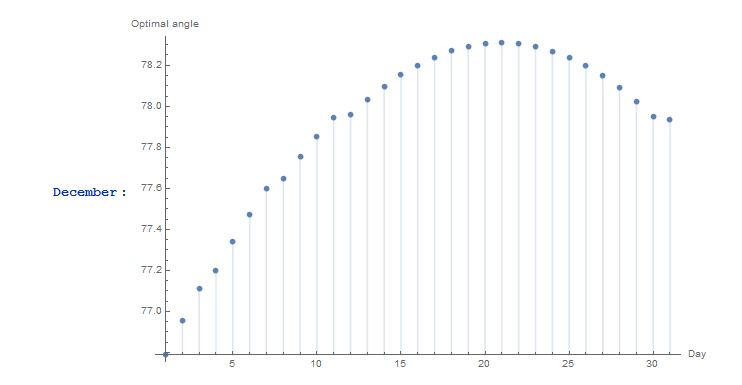
\includegraphics[width=0.8\textwidth]{graph_dec.JPG}
			   	\label{fig:graph_dec}
			   \end{figure}
			   \begin{figure}[h]
			   	\centering
			   	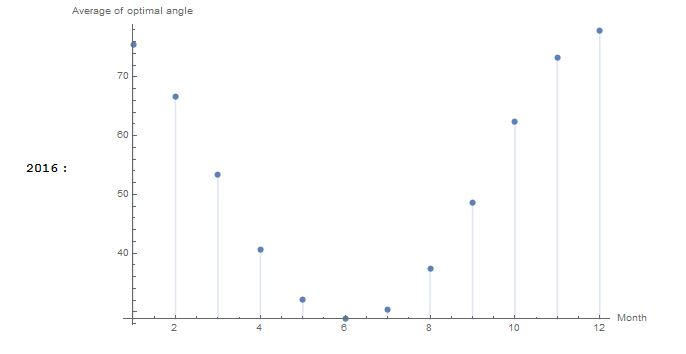
\includegraphics[width=0.8\textwidth]{graph_2016.JPG}
			   	\label{fig:graph_dec}
			   \end{figure}
			   	
\end{document}